\begin{frame}{}
    \vfill
       \center{\huge{
       \alert{I.\, Motivación}
       }}
    \vfill
\end{frame}
\begin{frame}{}
   \vfill\center\huge{¿Se pueden estudiar \alert{grafos} usando \alert{topología?}}\vfill
\end{frame}
{\usebackgroundtemplate{}
\begin{frame}
  \frametitle{Naturalmente\dots}
  \begin{tikzpicture}[remember picture, overlay]
    % Diagrama de los puentes (Fig. 1 de Euler)
    \node[anchor=north west, inner sep=0pt,
          xshift=0.06\paperwidth, yshift=-0.28\paperheight]
          at (current page.north west)
          {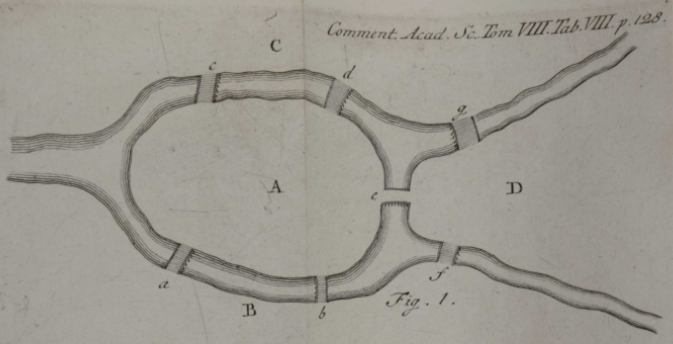
\includegraphics[width=0.45\paperwidth]{Images/Puentes.png}};
    % Retrato de Euler, encima del diagrama
    \node[anchor=north west, inner sep=0pt,
          xshift=0.345\paperwidth, yshift=-0.47\paperheight]
          at (current page.north west)
          {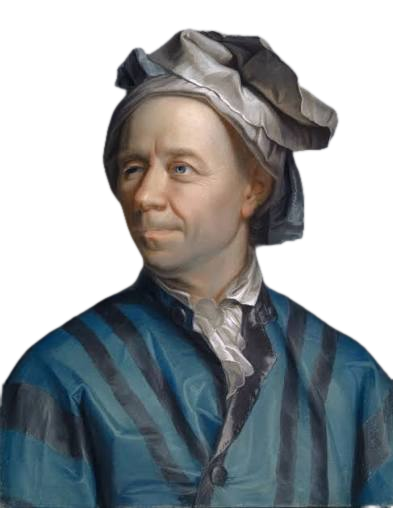
\includegraphics[width=0.18\paperwidth]{Images/Euler.png}};
    % Primera página del artículo
    \node[anchor=north west, inner sep=0pt,
          xshift=0.617\paperwidth, yshift=-0.238\paperheight]
          at (current page.north west)
          {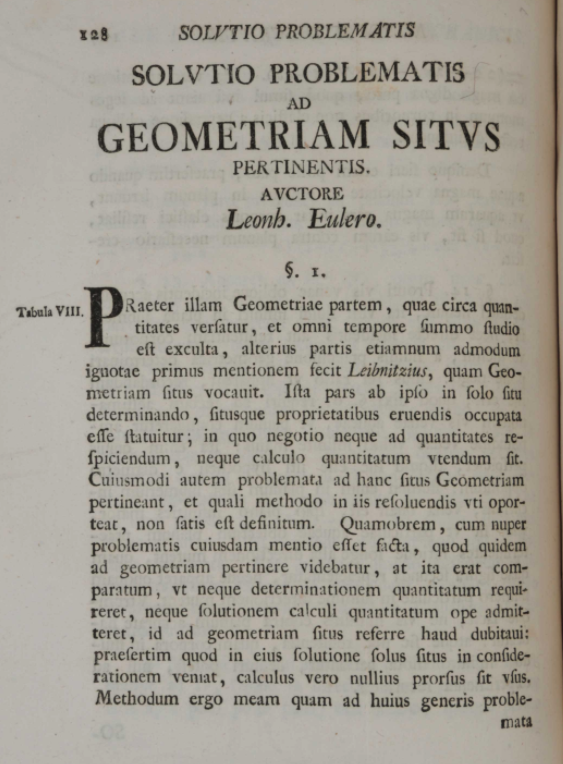
\includegraphics[width=0.285\paperwidth]{Images/Art_titulo.png}};
    % Pies de imagen
    \node[align=center, font=\footnotesize,
          xshift=0.286\paperwidth, yshift=-0.845\paperheight]
          at (current page.north west)
          {1736: Solución de L.~Euler del problema\\
           de los siete puentes de Königsberg};
    \node[align=center, font=\footnotesize,
          xshift=0.76\paperwidth, yshift=-0.845\paperheight]
          at (current page.north west)
          {``Solución de un problema relativo\\
           a la \alert{geometría de la posición}''};
  \end{tikzpicture}
\end{frame}}
\begin{frame}{Nuestro interés principal: grafos simples}
   \begin{columns}[c]
      \begin{column}{0.45\textwidth}
         \begin{Def}
            Un \textbf{grafo simple} es una pareja $G=(V,E)$ de conjuntos, donde los elementos de $E$ son subconjuntos de $V$, de exactamente dos elementos.\vspace{0.3cm}
         \end{Def}
      \end{column}
      \begin{column}{0.53\textwidth}
         \small
         \begin{itemize}
            \item<2-> Representamos $\{v_i,v_j\}$ por $v_iv_j$
            \item<3->[] \alert{Ejemplo:}
            \item<3-> $V=\{v_1,v_2,v_3,v_4,v_5\}$
            \item<3-> $G=(V,\{v_1v_2,v_2v_3,v_2v_4,v_2v_5\})$
         \end{itemize}
         \vspace{0.25cm}
         \centering
         \uncover<4->{\begin{tikzpicture}[
  vnode/.style={circle, fill=FancyBlue!40, draw=black, thick, text=black,
                minimum size=6mm, inner sep=0pt, font=\footnotesize}
]
  % Vértices: v2 en el centro
  \coordinate (v1) at (90:1.25);
  \coordinate (v2) at (0,0);
  \coordinate (v3) at (-45:1.25);
  \coordinate (v4) at (-90:1.25);
  \coordinate (v5) at (225:1.25);

  % Aristas: v1v2, v2v3, v2v4, v2v5
  \foreach \i in {1,3,4,5}
    \draw[thick] (v2) -- (v\i);

  \foreach \i in {1,...,5}
    \node[vnode] at (v\i) {$v_{\i}$};
\end{tikzpicture}
}
      \end{column}
   \end{columns}
\end{frame}\begin{frame}{Teoría topológica de grafos: la conexión más conocida}
   
\end{frame}
\begin{frame}{Nuestro enfoque: topologías de Alexandroff sobre $V$}
   \vspace{-0.3cm}
   \begin{Def}
      Topología sobre $X$:
      \begin{itemize}
         \item $\emptyset$ y $X$ son abiertos.
         \item Unión arbitraria de abiertos es abierto.
         \item \alert{Intersección finita} de abiertos es abierto.
      \end{itemize}\vspace{0.3cm}
   \end{Def}
   \uncover<2->{%
   \begin{Def}
      Topología de \alert{Alexandroff}: \alert{intersección arbitraria} de abiertos es abierto.\vspace{0.3cm}
   \end{Def}}
\end{frame}
{\usebackgroundtemplate{}
\begin{frame}{Motivación: topología digital}
   \centering
   \reflectbox{
\includegraphics[width=0.9\textwidth,height=\textheight,keepaspectratio]{Images/Tomografia.pdf}}
\end{frame}}

\begin{frame}{Propiedad clave}
   \begin{prop}
      Un espacio es de Alexandroff si y solo si todo punto tiene una \alert{vecindad mínima}.\vspace{0.3cm}
   \end{prop}
   \begin{center}
      \tikzset{every picture/.append style={scale=0.7}}
      \uncover<2->{\begin{tikzpicture}[
  abierto/.style={draw=black, thick, dashed}
]
  % Abiertos que contienen a x
  \def\abiertoA{[rotate around={20:(-0.8,0.35)}] (-0.8,0.35) ellipse (1.7 and 1.0)}
  \def\abiertoB{[rotate around={-25:(0.85,0.45)}] (0.85,0.45) ellipse (1.6 and 0.95)}
  \def\abiertoC{[rotate around={10:(0.2,-0.6)}] (0.2,-0.6) ellipse (1.15 and 1.45)}
  \def\abiertoD{[rotate around={-10:(-0.2,-0.1)}] (-0.2,-0.1) ellipse (2.9 and 2.1)}

  % U_x: intersección de todos los abiertos que contienen a x
  \begin{scope}
    \clip \abiertoA;
    \clip \abiertoB;
    \clip \abiertoC;
    \fill[FancyBlue!25] \abiertoD;
  \end{scope}

  \draw[abierto] \abiertoA;
  \draw[abierto] \abiertoB;
  \draw[abierto] \abiertoC;
  \draw[abierto] \abiertoD;

  % Punto x
  \fill (0.3,0.25) circle (1.5pt) node[left, yshift=3pt] {$x$};

  % Etiqueta de U_x
  \node (Ux) at (-3.6,1.9) {$U_x$};
  \draw[shorten >=2pt] (-0.29,0.74) to[out=150, in=0] (Ux.east);
\end{tikzpicture}
}
   \end{center}
\end{frame}
